\documentclass[12pt, a4paper]{article}


\usepackage{nameref}
\usepackage{amsmath}
\usepackage{wasysym}
\usepackage{amsthm}
\usepackage{amssymb}
\usepackage[utf8]{inputenc}
\usepackage[dutch]{babel}
\usepackage{graphicx}
\usepackage{float}
\usepackage{subfig}
\usepackage[a4paper, left=1in]{geometry}
\usepackage{xcolor}
\usepackage{booktabs} % Top and bottom rules for tables
\usepackage{hyperref}
\hypersetup{urlcolor={blue}, colorlinks=false, linkcolor=., citecolor=.}
\usepackage[backend=biber,style=authortitle-comp]{biblatex}
\usepackage{csquotes}

\setlength{\belowcaptionskip}{-5pt}

% prutsen met fonts, xelatex compiler nodig!
% \newcommand{\mainfont}{Humor-Sans.ttf}
% \usepackage{mathspec} %loads fontspec as well
% \setmainfont{\mainfont}
% \setmathrm{\mainfont}
% \setmathfont(Digits,Latin){\mainfont}

\newcommand{\du}{\,\mathrm{d}}
\newcommand{\bgtan}{\mathrm{\,Bgtan\,}}
\newcommand{\bgsin}{\mathrm{\,Bgsin\,}}
\newcommand{\bgcos}{\mathrm{\,Bgcos\,}}
\newcommand{\p}{\mathcal{P}}
\newcommand{\R}{\mathbb{R}}
\newcommand{\Z}{\mathbb{Z}}
\newcommand{\N}{\mathbb{N}}
\newcommand{\q}{\mathbb{Q}}
\newcommand{\BO}{\mathcal{O}}
\newcommand{\x}{\textbf{x}}

\theoremstyle{definition}
\newtheorem{oef}{Oefening}[subsection]

\title{Practicum differentiaalvergelijkingen: De Lorenz Attractor}
\author{Pieter Luyten}
\date{November 2018}

\begin{document}

\maketitle

\begin{figure}[H]
    \centering
    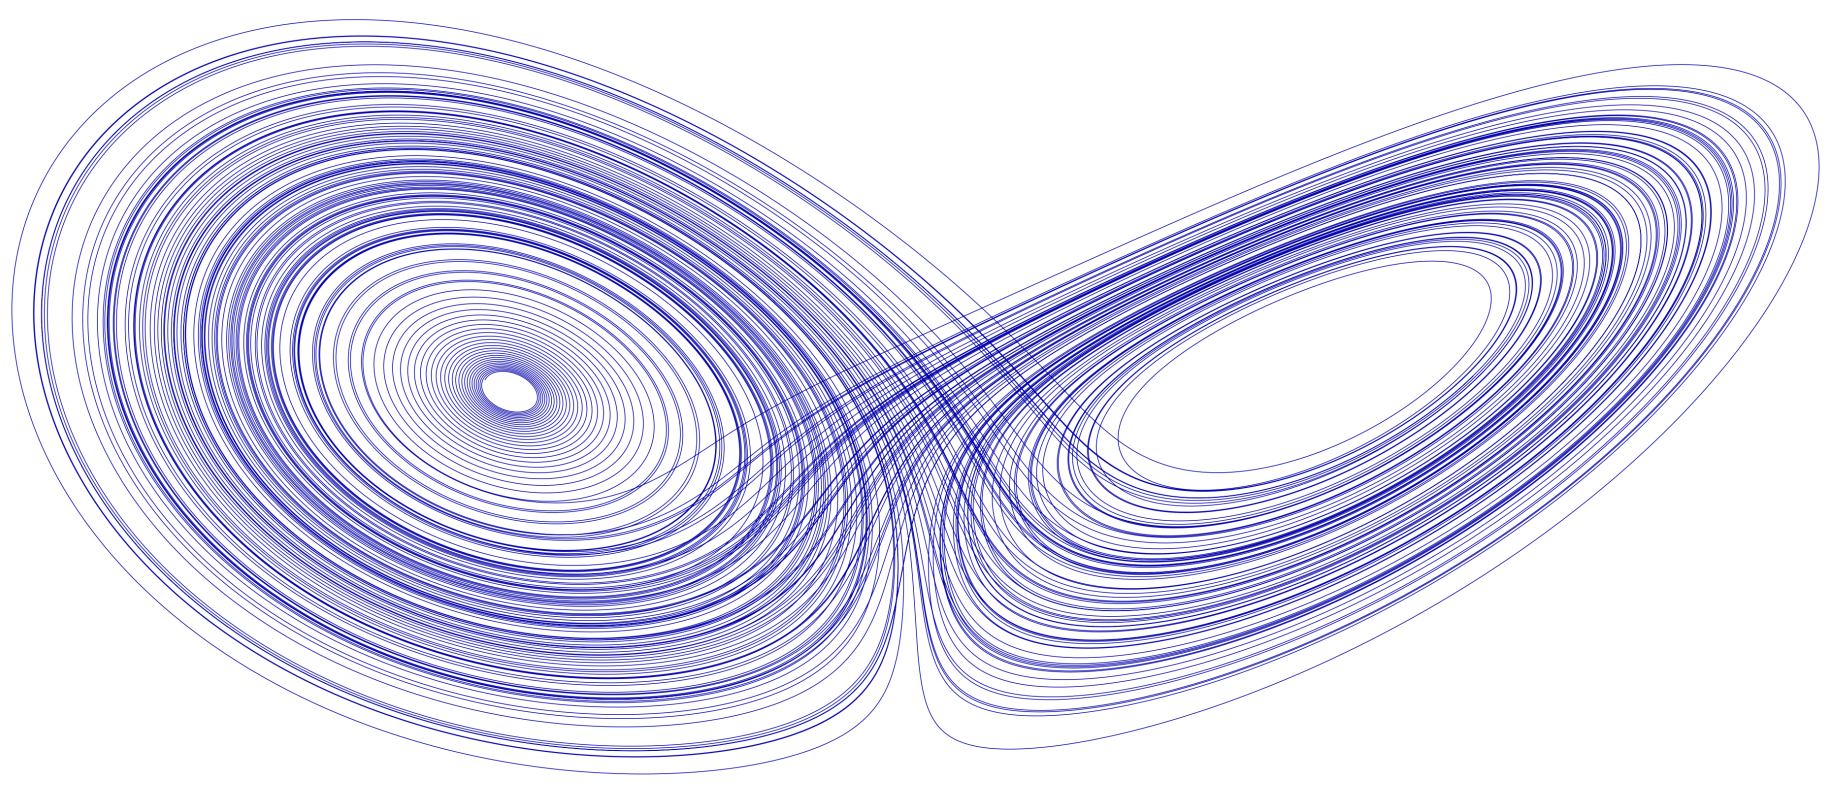
\includegraphics[width=0.9\linewidth]{header_verslag.png}
\end{figure}

\section{Inleiding}
In dit practicum bestuderen we het gedrag van de Lorenz attractor voor specifieke waarden voor de parameters. De Lorenz attractor wordt beschreven door een stelsel van 3 differentiaalvergelijkingen:
\begin{align}
    x'(t) &= -\sigma x + \sigma y \nonumber \\
    y'(t) &= r x -y -xz \label{eq:stelses_lorenz}\\
    z'(t) &= -bx +xy \nonumber
\end{align}

Hierin zijn $\sigma, r, b$ 3 reële parameters. We stellen deze voor de rest van dit document gelijk aan:
$$\sigma = 10 \qquad r=28 \qquad b = 8/3$$
Dit is een sterk vereenvoudigd model van het weer, een zogenaamd "speelgoedmodel". Dit werd voor het eerst bestudeerd door Edward Lorenz. Het is uit dit model dat de term vlindereffect is ontstaan. De oplossingen zijn over het algemeen heel chaotisch en een heel kleine aanpassing aan de beginvoorwaarde heeft na lange tijd een heel groot effect. De afbeelding in de header toont een pad op de Lorenz attractor, het oppervlak waar de oplossingen naar toe worden getrokken.\\
\\
Deze differentiaalvergelijking werd bestudeerd met numerieke methoden. Ik heb IJulia notebooks gebruikt voor de numerieke methoden om de vergelijking op te lossen en verdere analyse. Voor de analyse van de kritieke punten heb ik het package sympy gebruikt om met symbolische vergelijkingen te werken. De gebruikte code kan je \href{https://nbviewer.jupyter.org/github/Cubedsheep/practicum-diff-Julia/blob/master/practicum%20-%20Julia.ipynb?fbclid=IwAR0w5uD6396VRiiF5jM1AxzXG7EB4HG5WAsDRnNsDRpx_s_2yaZP3bjLWWA}{hier
} vinden.



\section{Kritieke punten}
We berekenen eerst de kritieke punten van het systeem van differentiaalvergelijkingen. Dit zijn punten waarin elke vergelijking van het stelsel gelijk is aan 0. In dit geval zijn er 3 kritieke punten: de oorsprong ($O$), een punt met negatieve $x$-coördinaat ($A$) en een punt met positieve $x$-coördinaat ($B$). De coördinaten van de kritieke punten zijn:
\begin{align*}
    O &= \left ( 0, \quad 0, \quad 0\right )\\
    A &= \left ( - 6 \sqrt{2}, \quad - 6 \sqrt{2}, \quad 27\right )\\
    B &= \left ( 6 \sqrt{2}, \quad 6 \sqrt{2}, \quad 27\right )
\end{align*}
Voor de analyse van de kritieke punten bepalen we de eigenwaarden en bijhorende eigenvectoren van de Jacobiaan in deze punten. Dit geeft:
\begin{align*}
    A: \lambda_1 &= -13.85, \Vec{v_1} = \left[ \begin{array}{cc}0.85 \\ -0.32 \\ 0.39\end{array} \right]; \lambda_2 = 0.0939 + 10.1945i, \Vec{v_2} = \left[ \begin{array}{c} -0.26-0.29i \\ 0.032-0.56i \\ 0.719 \end{array} \right];\\
    \lambda_3 &= 0.0939 - 10.1945i, \Vec{v_2} = \left[ \begin{array}{c} -0.26+0.29i \\ 0.032+0.56i \\ 0.719 \end{array} \right]\\
    B: \lambda_1 &= -13.85, \Vec{v_1} = \left[ \begin{array}{cc}0.85 \\ -0.32 \\ -0.39\end{array} \right]; \lambda_2 = 0.0939 + 10.1945i, \Vec{v_2} = \left[ \begin{array}{c} -0.26-0.29i \\ 0.032-0.56i \\ -0.719 \end{array} \right];\\
    \lambda_3 &= 0.0939 - 10.1945i, \Vec{v_2} = \left[ \begin{array}{c} -0.26+0.29i \\ 0.032+0.56i \\ -0.719 \end{array} \right]\\
    O: \lambda_1 &= -22.827, \Vec{v_1} = \left[\begin{array}{c} -0.614\\  0.788\\ 0\end{array} \right]; \lambda_2 = 11.827, \Vec{v_2} = \left[ \begin{array}{c} -0.416\\-0.909\\0\end{array}\right];
    \lambda_3 = -\frac{8}{3}, \Vec{v_3} = \left[ \begin{array}{c}0\\0\\1\end{array} \right]
\end{align*}
Bij de punten $A$ en $B$ zien we dat er 1 negatieve en 2 complexe eigenwaarden zijn. De eigenwaarde $\lambda_1$ is negatief, de oplossingen zullen naar de punten getrokken worden in de richting van $\Vec{v_1}$. De eigenwaarden bij de andere 2 eigenvectoren zijn complex, in het vlak opgespannen door (de reële delen van) deze eigenvectoren hebben we een spiraalpunt. Dit is een onstabiel spiraalpunt omdat het reële deel van de eigenwaarden positief is. \\
\\
In het punt $O$ zijn er 3 reële eigenwaarden, 1 negatief en 2 positief, de component van de richtingsvector volgens $\Vec{v_1}$ zal dus negatief zijn en de oplossingen naar het vlak door $O$ opgespannen door $\Vec{v_2}$ en $\Vec{v_3}$ trekken. In dit vlak hebben we een bron want de eigenwaarden bij de 2 eigenvectoren in dit vlak zijn positief. Dit kritiek punt is dus niet stabiel en zeker niet asymptotisch stabiel.\\
\\
We zien dus dat de oplossingen naar de vlakken opgespannen door de complexe eigenvectoren van de Jacobiaan in $A$ en $B$ worden getrokken. In de buurt van het onstabiele kritieke punt $O$ kunnen ze van vlak wisselen.



\section{Periodische oplossingen}
Hoewel het gedrag van de oplossingen van vergelijking [1] in het algemeen chaotisch is, zijn er oplossingen met specifieke beginvoorwaarden die een periodiek gedrag vertonen. Dit periodiek gedrag duiden we aan met een sequentie van A's en B's die zegt hoe vaak en in welke volgorde de oplossing rond elk punt draait.

\subsection{Oplossing AB}
Voor de beginvoorwaarde $\textbf{x}(0)$:
$$x(0) =−13,763 610 682 134, \quad y(0) =−19,578 751 942 452, \quad   z(0) = 27$$
vinden we een periodieke oplossing AB. Deze draait dus een keer rond A, een keer rond B en komt dan terug op de beginwaarde uit. Deze beginwaarde kunnen we gebruiken om de nauwkeurigheid van numerieke methodes te testen. We benaderen de oplossing met 3 numerieke methodes: de methode van Euler, de verbeterde methode van Euler en Runge-Kutta van orde 4. Voor elke methode zoeken we dan de stapgrootte die nodig is om de fout op de eindwaarde kleiner dan $10^{-5}$ te krijgen.\\
\\
De functies om de oplossing numeriek te benaderen geven als return value een lijst met opeenvolgende punten van de oplossing. In deze lijst zoeken we het punt dat het dichtst bij de beginwaarde ligt, noem dit punt $D$, het punt ervoor $C$ en het punt na $D$ noemen we $E$. Deze afstand is echter niet altijd de kleinste afstand tot de beginwaarde, hiervoor moeten we de afstand van de beginwaarde tot de lijnstukken $[CD]$ en $[DE]$ ook bepalen. Als deze afstand kleiner is, en de loodrechte projectie van de beginwaarde op dit lijnstuk ligt, is dit de kleinste afstand tot de beginwaarde. Als de 2 loodrechte projecties niet op het lijnstuk liggen, gebruiken we de tijd tot het dichtste punt als benadering van de periode. In het andere geval projecteren we $\textbf{x}(0)$ op het lijnstuk waar het het dichtste bij ligt, noem deze projectie $P$. We berekenen dan de verhouding $-\frac{|DP|}{|CD|}$ of $\frac{|DP|}{|DE|}$. Dit vermenigvuldigen we met de stapgrootte $h$ en tellen we op bij de tijd tot het punt $D$ om een schatting voor de periode $T$ van de periodische baan te krijgen. De min bij $-\frac{|DP|}{|CD|}$ staat er omdat dit punt "voor" het punt $D$ ligt als je de oplossingskromme doorloopt\\
Deze methode geeft volgende waardes voor $h$ en $T$ zodat $|\textbf{x}(0) - \textbf{x}(T)| < 10^{-5}$
\begin{align*}
\text{methode van Euler}: & h = 3 \cdot 10^{-7} & \, T = 1,5586, &\, \text{afwijking} = 7,26 \cdot 10^{-6}\\
\text{verbeterde methode van Euler}: & \, h = 8 \cdot 10^{-4} &\, T = 1,55864188, & \text{afwijking} = 8,77 \cdot 10^{-6}\\
\text{Runge-Kutta van orde 4}: &\, h = 3 \cdot 10^{-4} & T = 1,55865233, &\, \text{afwijking} = 8,48 \cdot 10^{-6}
\end{align*}
De differentiaalvergelijking heel exact benaderen met Runge-Kutta van orde 4 en stapgrootte $10^{-7}$ geeft een periode van $T=1.558 \, 652 \, 210$. In figuur [1] zie je de projectie van de periodische oplossing op het $xz$-vlak.

\begin{figure}[H]
    \centering
    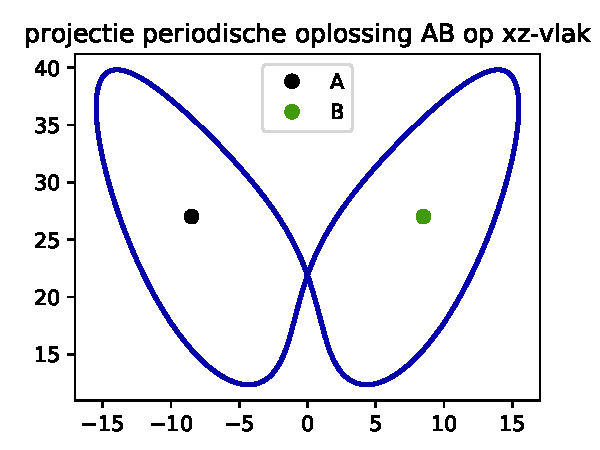
\includegraphics[width=0.5\linewidth]{projectie_opdracht_3.pdf}
    \caption{De projectie in het xz-vlak van een periodische oplossing AB}
    \label{fig: AB}
\end{figure}

\subsection{Oplossing AAAB}
Er is gegeven dat voor de beginwaarden
\begin{equation}
x(0) =−11, 998 523 280 062, \quad y(0) \in [-16, -15] \quad   z(0) = 27
\label{eq: AAAB-x0}
\end{equation}
er een periodische oplossing is van de vorm AAAB. Het gedrag van de oplossingen is chaotisch maar we kunnen wel de continuïteit in de beginvoorwaarde gebruiken. Dit wordt analoog bewezen als de continuïteit in de beginvoorwaarde van 1 differentiaalvergelijking.\\
\\
Stel dat we een stelsel hebben van de vorm $\textbf{x}'(t) = \textbf{f}(t, \textbf{x})$ met $\textbf(f)$ continu op $[a, A] \times D$ en uniform Lipschitz continu op $D$. Stel dat $\textbf{x}_1$ en $\textbf{x}_2$ oplossingen zijn van de differentiaalvergelijking zodat voor alle $t \in [a, A]$ geldt dat $y_1, y_2 \in D$. Dan bestaat er voor elke $\epsilon > 0$ een $\delta > 0$ zodat $||\x_1(t)-\x_2(t)|| < \epsilon$ voor alle $t \in [a, A]$ volgt uit $||\x_1(a)-\x_2(a)|| < \delta$.

\begin{proof}
Stel $\phi(x) = ||\x_1(t) - \x_2(t)||^2$. voor de afgeleide geldt als $\x_1(t) \neq \x_2(t)$ dat:
\begin{align*}
\phi'(t) &\leq 2||\x_1(t) - \x_2(t)|| \, ||\x'_1(t) - \x'_2(t)||\\
 &= 2||\x_1(t) - \x_2(t)|| \, ||\textbf{f}(t, \x_1) - \textbf{f}(t, \x_2)||\\
 &\leq 2K||\x_1(t) - \x_2(t)||^2
 &= 2K \phi(x)
\end{align*}
Als norm gebruiken we de euclidische norm, deze is overal afleidbaar behalve in $0$, maar omdat we $\x_1(t) \neq \x_2(t)$ veronderstellen kunnen we de kettingregel toepassen. In de laatste stap gebruiken we de Lipschitz-continuïteit van $\mathbf{f}$ op $D$ en is $K$ de Lipschitz-constante. We kunnen nu het Lemma van Gronwall gebruiken op de functies $\phi(x)$ en $g(x) = 2K$ Dit geeft dan dat:
$$0 \leq \phi(x) \leq \phi(a) \exp(2K(t-a)).$$
Hieruit volgt dan dat:
$$ ||\x_1(t) - \x_2(t)|| \leq ||\x_1(a) - \x_2(a)|| \exp(K(A-a)) $$
stel $\delta = \epsilon \exp(-K(a-A))$, dan volgt het gevraagde voor $\x_1 \neq \x_2$. In het geval dat $\x_1(t) = \x_2(t)$ voor minstens 1 $t$ volgt uit de uniciteit van de oplossing dat $\x_1 = \x_2$, in dit geval geldt zeker het gevraagde.
\end{proof}
De differentiaalvergelijking van het model van Lorenz heeft een continue afgeleide over heel $\R^3$. Als we $t\in [0, T]$ bekijken zal de oplossing begrensd blijven, Deze ligt dus in een gesloten gebied $D$. Omdat $D$ gesloten is zal in elk punt elke richtingsafgeleide begrensd blijven, en kunnen we deze afschatten met 1 $K$. Dan volgt dat $\mathbf{f}$ Lipschitz continu is door voor elke $\x, \mathbf{y}$ de rechte tussen $\x, \mathbf{y}$ te bekijken en de richtingsafgeleide langs deze rechte.\\
\\
Dit kunnen we gebruiken om de periodische oplosing te zoeken. Eerst berekenen we voor 10 beginvoorwaarden in het interval [2] de oplossing en de afstand tot de beginwaarde in functie van de tijd. Dit kan je zien in de linkse grafiek van figuur [2]. Het is duidelijk dat vooral de rode, groene en oranje grafiek de beginwaarde terug dicht naderen rond $T=3$ na 2 lussen rond $A$.

\begin{figure}[h]
    \centering
    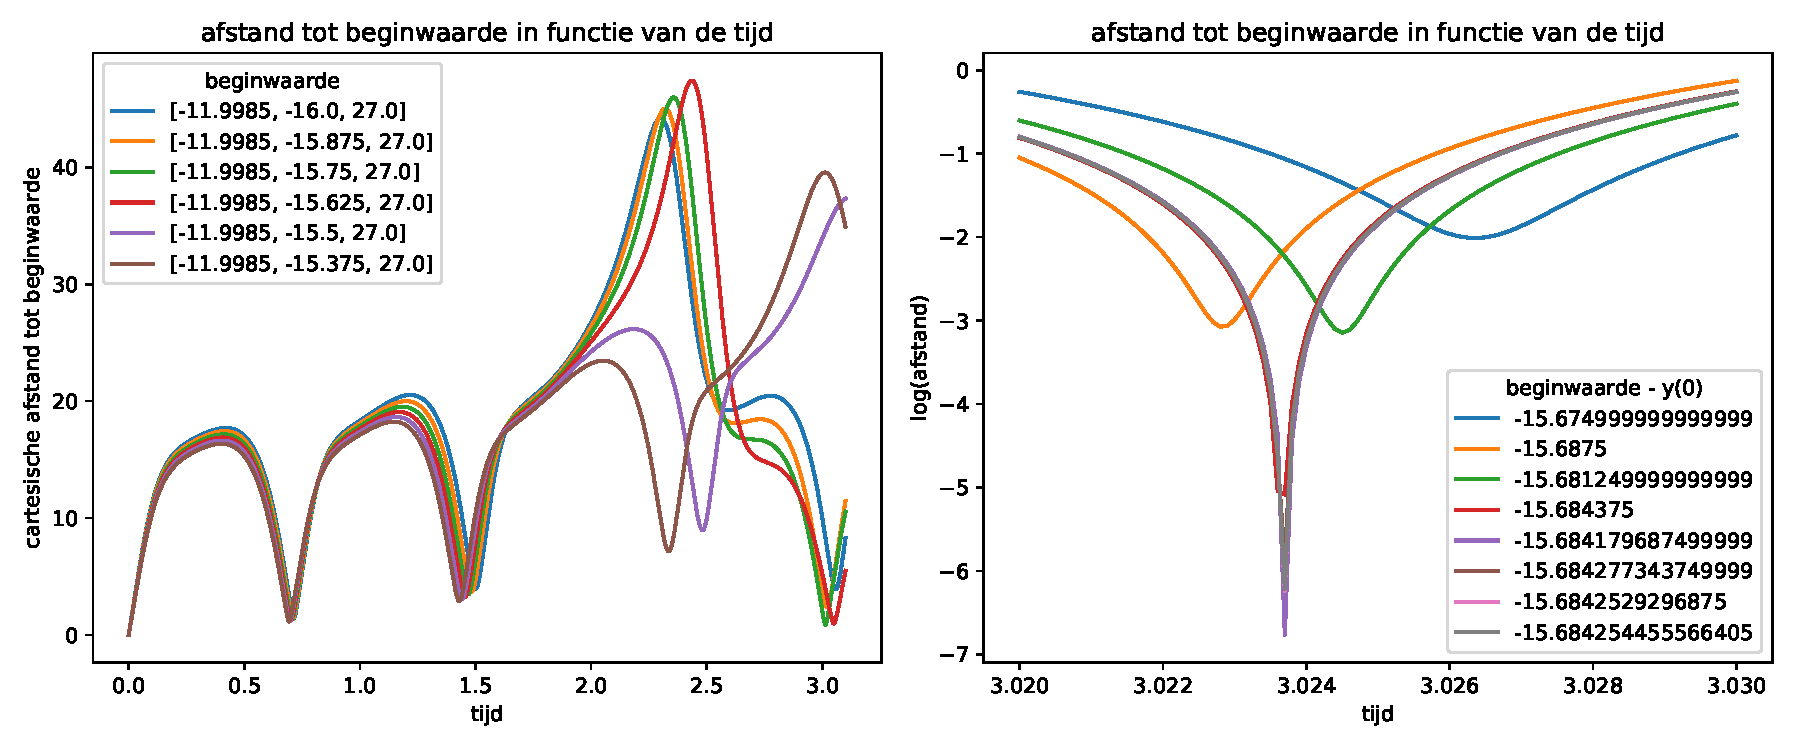
\includegraphics[width=\linewidth]{afstand_beginwaarde_opdracht4.pdf}
    \caption{Links: afstand tot de beginwaarde in functie van de tijd voor een aantal beginwaarden met $y(0) \in [-16, -15]$. Rechts: de afstand tot de beginwaarde in functie van de tijd, rond het tijdstip waarop de oplossing het dichtst komt voor opeenvolgende iteraties van de verfijningsmethode}
    \label{fig: afstand}
\end{figure}

 We zetten nu een iteratieproces op waarbij we steeds 5 oplossingen bekijken. Nummer deze $\x_i$ zodat als $i<j$ dan $y_i(0) < y_j(0)$. Van deze 5 oplossingen zoeken we de oplossing die rond $T=3$ het dichtst (zijn) beginwaarde terug benadert, stel dat dit $\x_i$ is. In de volgende iteratiestap stellen we $y_1(0) = y_{i-1}(0), y_3(0) = y_i(0), y_5(0)=y_{i+1}(0)$. Indien $i \in \{1,5\}$ stel dan $i$ gelijk aan $2$ respectievelijk $4$. We berekenen nu steeds 2 nieuwe oplossingen met als $y$-waarde voor de beginwaarde $$y_2(0) = \frac{y_3(0)-y_1(0)}{2}, \quad y_4(0) = \frac{y_5(0)-y_3(0)}{2}$$\\
\\
Via dit iteratieproces vinden we de opeenvolgende $y$-waarden in de rechtse grafiek van figuur [2] en dat de periode iets minder dan 3,024 is. Het iteratieproces nog verder doorzetten geeft volgende waarden voor de beginwaarde voor y en de periode van de oplossing:
$$y_0 = -15,684\, 254 \, 098 , \quad T=3,023 \, 583 \, 703$$
Figuur [3] toont een plot van de periodische oplossing.

\begin{figure}[h]
    \centering
    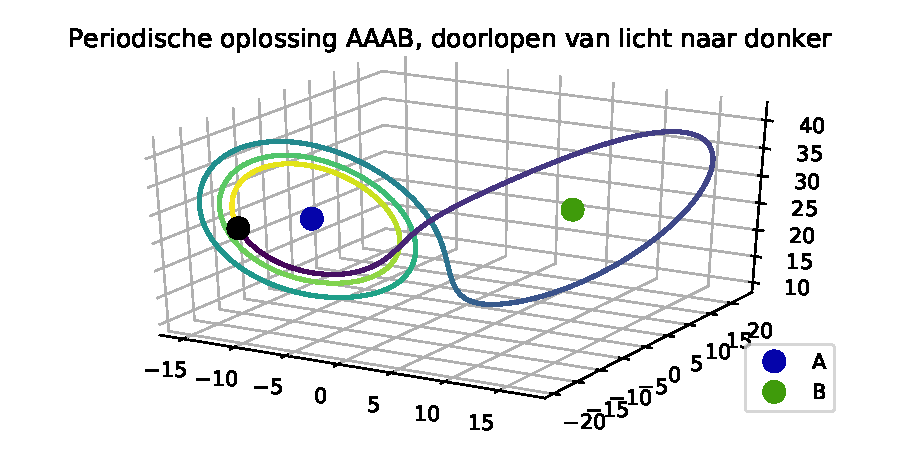
\includegraphics[width=0.8\linewidth]{periodische_baan_AAAB_opdracht4.pdf}
    \caption{Plot van een periodische baan AAAB. De kromme wordt doorlopen van geel naar paars (licht naar donker)}
    \label{fig: AAAB}
\end{figure}

\section{Vorm van de Lorenz attractor}
Nu plotten we een oplossing op de Lorenz attractor over een heel lange tijd om een idee te krijgen van de vorm van het oppervlak. In fiuur [4] zie je een oplossing met $t \in [0, 1500]$ geprojecteerd op de 3 coördinaatvlakken en een 3d-projectie. We zien duidelijk dat heel dicht bij de kritieke punten $A$ en $B$, en verder van de punten vandaan de banen steeds minder dicht zijn. Ook valt op dat de banen in de vlakken rond de kritieke punten blijven en wisselen van vlak in het kritieke punt $0$.

\begin{figure}
    \centering
    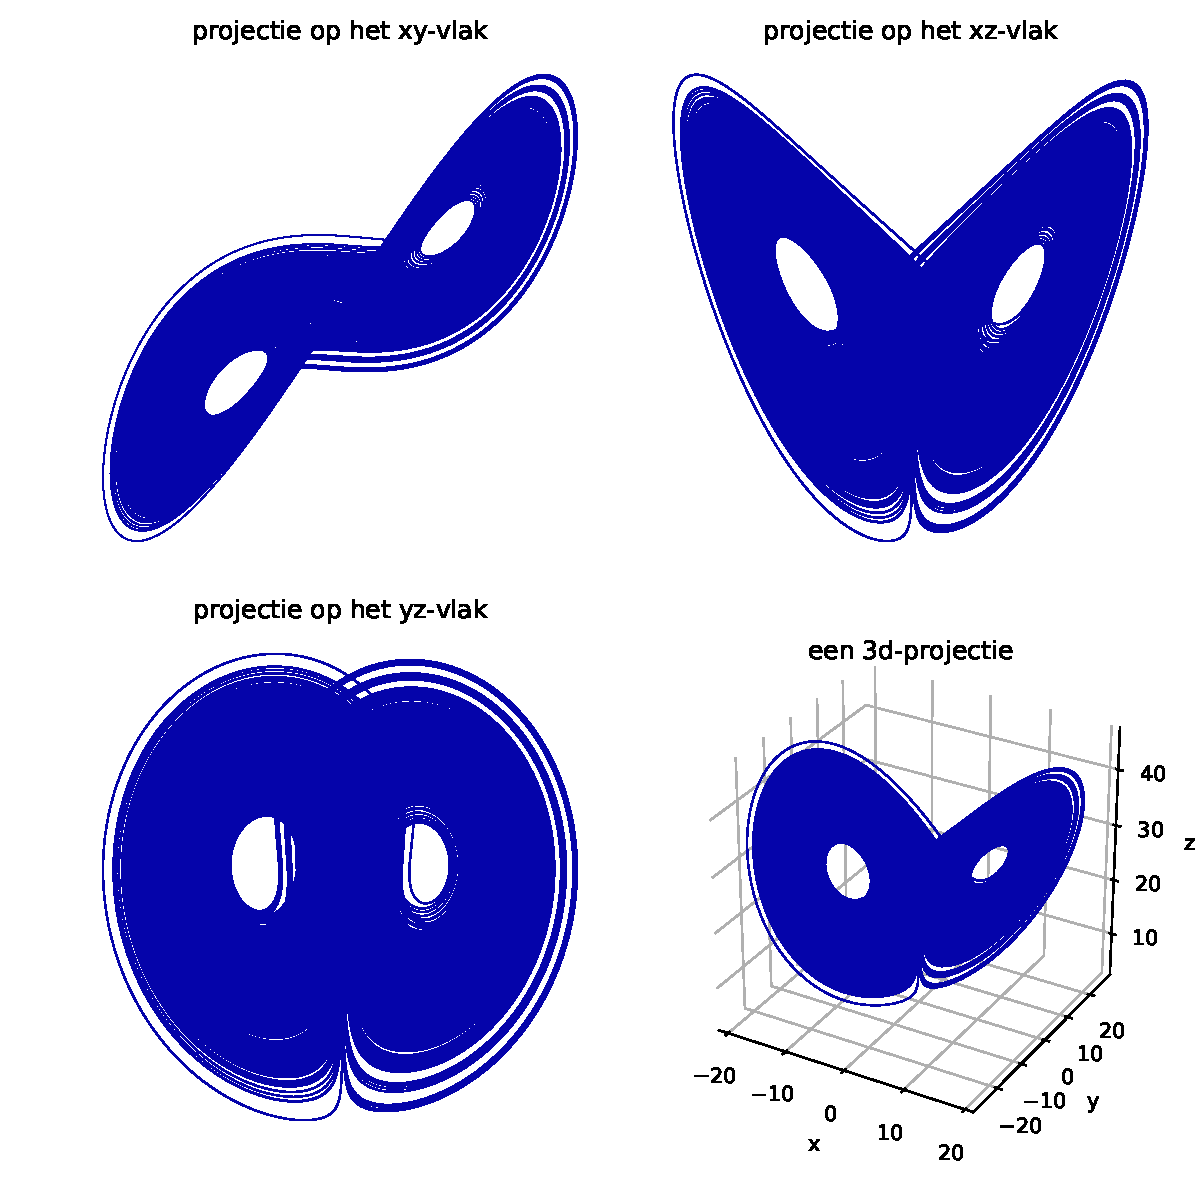
\includegraphics[width=0.9\linewidth]{projecties_opdracht_5.pdf}
    \caption{Projecties van een pad op de Lorenz attractor voor $T \rightarrow \infty$}
    \label{fig: projecties}
\end{figure}

\end{document}
